\documentclass[UTF8,a4paper,landscape]{ctexart}\usepackage[]{graphicx}\usepackage[]{color}
% maxwidth is the original width if it is less than linewidth
% otherwise use linewidth (to make sure the graphics do not exceed the margin)
\makeatletter
\def\maxwidth{ %
  \ifdim\Gin@nat@width>\linewidth
    \linewidth
  \else
    \Gin@nat@width
  \fi
}
\makeatother

\definecolor{fgcolor}{rgb}{0.345, 0.345, 0.345}
\newcommand{\hlnum}[1]{\textcolor[rgb]{0.686,0.059,0.569}{#1}}%
\newcommand{\hlstr}[1]{\textcolor[rgb]{0.192,0.494,0.8}{#1}}%
\newcommand{\hlcom}[1]{\textcolor[rgb]{0.678,0.584,0.686}{\textit{#1}}}%
\newcommand{\hlopt}[1]{\textcolor[rgb]{0,0,0}{#1}}%
\newcommand{\hlstd}[1]{\textcolor[rgb]{0.345,0.345,0.345}{#1}}%
\newcommand{\hlkwa}[1]{\textcolor[rgb]{0.161,0.373,0.58}{\textbf{#1}}}%
\newcommand{\hlkwb}[1]{\textcolor[rgb]{0.69,0.353,0.396}{#1}}%
\newcommand{\hlkwc}[1]{\textcolor[rgb]{0.333,0.667,0.333}{#1}}%
\newcommand{\hlkwd}[1]{\textcolor[rgb]{0.737,0.353,0.396}{\textbf{#1}}}%
\let\hlipl\hlkwb

\usepackage{framed}
\makeatletter
\newenvironment{kframe}{%
 \def\at@end@of@kframe{}%
 \ifinner\ifhmode%
  \def\at@end@of@kframe{\end{minipage}}%
  \begin{minipage}{\columnwidth}%
 \fi\fi%
 \def\FrameCommand##1{\hskip\@totalleftmargin \hskip-\fboxsep
 \colorbox{shadecolor}{##1}\hskip-\fboxsep
     % There is no \\@totalrightmargin, so:
     \hskip-\linewidth \hskip-\@totalleftmargin \hskip\columnwidth}%
 \MakeFramed {\advance\hsize-\width
   \@totalleftmargin\z@ \linewidth\hsize
   \@setminipage}}%
 {\par\unskip\endMakeFramed%
 \at@end@of@kframe}
\makeatother

\definecolor{shadecolor}{rgb}{.97, .97, .97}
\definecolor{messagecolor}{rgb}{0, 0, 0}
\definecolor{warningcolor}{rgb}{1, 0, 1}
\definecolor{errorcolor}{rgb}{1, 0, 0}
\newenvironment{knitrout}{}{} % an empty environment to be redefined in TeX

\usepackage{alltt} 
% 英文字体配置部分
%\setmainfont{Arial}
%\setsansfont{Source Sans Pro}
%\setmonofont{Source Code Pro}
% 中文字体配置部分
%\usepackage{xeCJK}%中文字体
%\setCJKmainfont[ItalicFont={楷体}, BoldFont={黑体}]{宋体}
%\setCJKsansfont{黑体}
%\setCJKmonofont{仿宋_GB2312}%中文等宽字体

\usepackage{fullpage}
\usepackage{pdflscape}
\usepackage{geometry}
\usepackage{needspace}
\usepackage{texshade}
\geometry{verbose,tmargin=1.8cm,bmargin=1.8cm,lmargin=1.8cm,rmargin=1.8cm}
\IfFileExists{upquote.sty}{\usepackage{upquote}}{}
\begin{document}



\subsection*{Chromatogram}
\begin{knitrout}
\definecolor{shadecolor}{rgb}{0.969, 0.969, 0.969}\color{fgcolor}
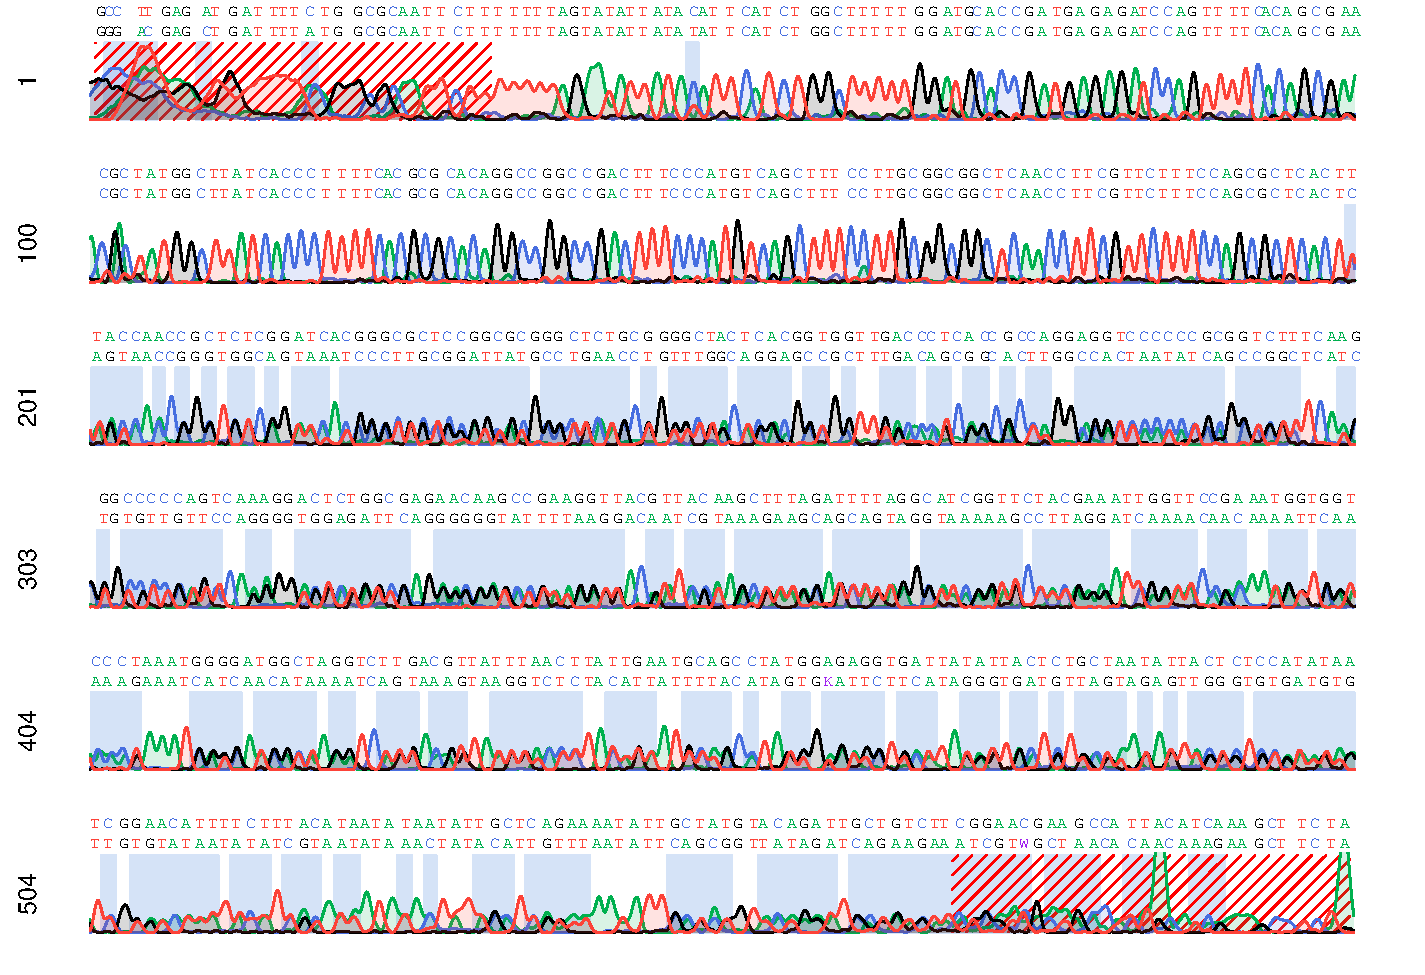
\includegraphics[width=\maxwidth]{figure/chromatogram-1} 

\end{knitrout}

\newpage

\subsection*{Alignment}
% Alignment of gsub("\\$|_", "\\.", input$seq$name) sequence data to
% inputdata()$note$refname reference sequence.
\begin{knitrout}
\definecolor{shadecolor}{rgb}{0.969, 0.969, 0.969}\color{fgcolor}\begin{kframe}
\begin{verbatim}


Alt Allele         1 CGCCCCGCCGCCCTCCCCAGAGCCCCGGTGCCTCACCTCACCAGCGTGGCCTCCCCCGAGTACTTGAGGTCTTCCAGCTC     80
                     ||||||||||||||||||||||||||||||||||||||||||||||||||||||||||||||||||||||||||||||||
Reference         31 CGCCCCGCCGCCCTCCCCAGAGCCCCGGTGCCTCACCTCACCAGCGTGGCCTCCCCCGAGTACTTGAGGTCTTCCAGCTC    110

Alt Allele        81 CCGCTGCAGTTGTTGCTTCTCCTGCTTCAGCCTCACCAACGTCTGCTCGTTCTCGCTCTTGAGCGTCTCCAACTGCGCGA    160
                     ||||||||||||||||||||||||||||||||||||||||||||||||||||||||||||||||||||||||||||||||
Reference        111 CCGCTGCAGTTGTTGCTTCTCCTGCTTCAGCCTCACCAACGTCTGCTCGTTCTCGCTCTTGAGCGTCTCCAACTGCGCGA    190

Alt Allele       161 AGGTGTCGCCCTGGGCCAGGAACCGCCGCACCAACGACTGCGGGCCACCCAGCCCCAGTCAGAGCCAGGGCCTAGGGAGC    240
                     ||||||||||||||||||||||||||||||||||||||||||||||||||||||||||||||||||||||||||||||||
Reference        191 AGGTGTCGCCCTGGGCCAGGAACCGCCGCACCAACGACTGCGGGCCACCCAGCCCCAGTCAGAGCCAGGGCCTAGGGAGC    270

Alt Allele       241 GTAGGGGCGCTCCACCTCCTCTCCCCCACCCTGCGAACCCTCGCACGCAGGACAGGTGGCCTGAGCTGGCGCCTTTTGCA    320
                     ||||||||||||||||||||||||||||||||||||||||||||||||||||||||||||||||||||||||||||||||
Reference        271 GTAGGGGCGCTCCACCTCCTCTCCCCCACCCTGCGAACCCTCGCACGCAGGACAGGTGGCCTGAGCTGGCGCCTTTTGCA    350

Alt Allele       321 CAGCAATGTATGGGGACACTGTGGGTTGGACGCAGGGTTGCTTCAAGGGTGAGCAGCCCTGGATATATCATTTTTGCGGG    400
                     ||||||||||||||||||||||||||||||||||||||||||||||||||||||||||||||||||||||||||||||||
Reference        351 CAGCAATGTATGGGGACACTGTGGGTTGGACGCAGGGTTGCTTCAAGGGTGAGCAGCCCTGGATATATCATTTTTGCGGG    430

Alt Allele       401 GCCCTTTCTGGCCTATA    417
                     |||||||||||||||||
Reference        431 GCCCTTTCTGGCCTATA    447
\end{verbatim}
\end{kframe}
\end{knitrout}

\subsection*{Alternative allele}
\begin{knitrout}
\definecolor{shadecolor}{rgb}{0.969, 0.969, 0.969}\color{fgcolor}\begin{kframe}
\begin{verbatim}
CGCCCCGCCGCCCTCCCCAGAGCCCCGGTGCCTCACCTCACCAGCGTGGCCTCCCCCGAGTACTTGAGGTCTTCCAGCTCCCGCTGCAGTTGTTGCTTCTCCTGCTTCAGCCTCACCAAC
GTCTGCTCGTTCTCGCTCTTGAGCGTCTCCAACTGCGCGAAGGTGTCGCCCTGGGCCAGGAACCGCCGCACCAACGACTGCGGGCCACCCAGCCCCAGTCAGAGCCAGGGCCTAGGGAGC
GTAGGGGCGCTCCACCTCCTCTCCCCCACCCTGCGAACCCTCGCACGCAGGACAGGTGGCCTGAGCTGGCGCCTTTTGCACAGCAATGTATGGGGACACTGTGGGTTGGACGCAGGGTTG
CTTCAAGGGTGAGCAGCCCTGGATATATCATTTTTGCGGGGCCCTTTCTGGCCTATA
\end{verbatim}
\end{kframe}
\end{knitrout}

\subsection*{Reference sequence}
\begin{knitrout}
\definecolor{shadecolor}{rgb}{0.969, 0.969, 0.969}\color{fgcolor}\begin{kframe}
\begin{verbatim}
WTGCTGACAGYAGTCCCCGGGGGCTCAGCCCGCCCCGCCGCCCTCCCCAGAGCCCCGGTGCCTCACCTCACCAGCGTGGCCTCCCCCGAGTACTTGAGGTCTTCCAGCTCCCGCTGCAGT
TGTTGCTTCTCCTGCTTCAGCCTCACCAACGTCTGCTCGTTCTCGCTCTTGAGCGTCTCCAACTGCGCGAAGGTGTCGCCCTGGGCCAGGAACCGCCGCACCAACGACTGCGGGCCACCC
AGCCCCAGTCAGAGCCAGGGCCTAGGGAGCGTAGGGGCGCTCCACCTCCTCTCCCCCACCCTGCGAACCCTCGCACGCAGGACAGGTGGCCTGAGCTGGCGCCTTTTGCACAGCAATGTA
TGGGGACACTGTGGGTTGGACGCAGGGTTGCTTCAAGGGTGAGCAGCCCTGGATATATCATTTTTGCGGGGCCCTTTCTGGCCTATATAAGGAATTTGAGTCAGCCTCAAACTCGAT
\end{verbatim}
\end{kframe}
\end{knitrout}

\subsection*{Alignment parameters}
\begin{knitrout}
\definecolor{shadecolor}{rgb}{0.969, 0.969, 0.969}\color{fgcolor}\begin{kframe}
\begin{verbatim}
########################################
# Program: Biostrings (version 2.56.0), a Bioconductor package
# Rundate: Mon Sep 14 23:00:37 2020
########################################
#=======================================
#
# Aligned_sequences: 2
# 1: Alt Allele
# 2: Reference
# Matrix: NA
# Gap_penalty: 12.0
# Extend_penalty: 2.0
#
# Length: 417
# Identity:     417/417 (100.0%)
# Similarity:    NA/417 (NA%)
# Gaps:           0/417 (0.0%)
# Score: 1070.318
\end{verbatim}
\end{kframe}
\end{knitrout}

\newpage

\subsection*{Chromatogram2(height=2,width=manual)}
\begin{knitrout}
\definecolor{shadecolor}{rgb}{0.969, 0.969, 0.969}\color{fgcolor}
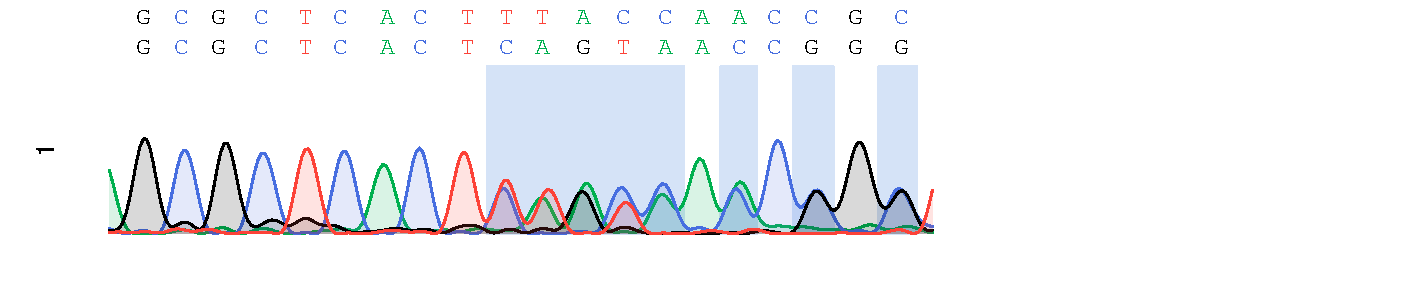
\includegraphics[width=\maxwidth]{figure/chromatogram2-1} 

\end{knitrout}

\subsection*{Chromatogram3(height=1.6,width=40)}
\begin{knitrout}
\definecolor{shadecolor}{rgb}{0.969, 0.969, 0.969}\color{fgcolor}\begin{kframe}


{\ttfamily\noindent\bfseries\color{errorcolor}{\#\# Error in par(originalpar): 图形参数"{}pin"{}的值设得不对}}\end{kframe}
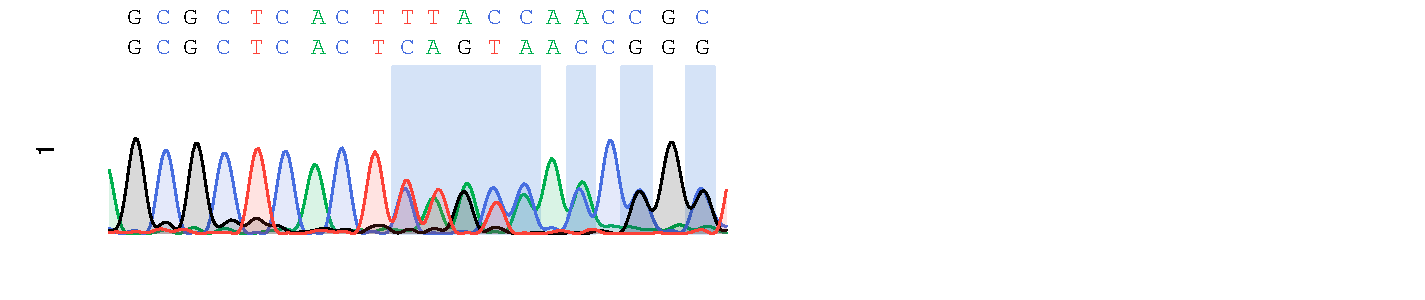
\includegraphics[width=\maxwidth]{figure/chromatogram3-1} 

\end{knitrout}

@

\subsection*{Chromatogram4(height=1.6,width=50)}
\begin{knitrout}
\definecolor{shadecolor}{rgb}{0.969, 0.969, 0.969}\color{fgcolor}\begin{kframe}


{\ttfamily\noindent\bfseries\color{errorcolor}{\#\# Error in par(originalpar): 图形参数"{}pin"{}的值设得不对}}\end{kframe}
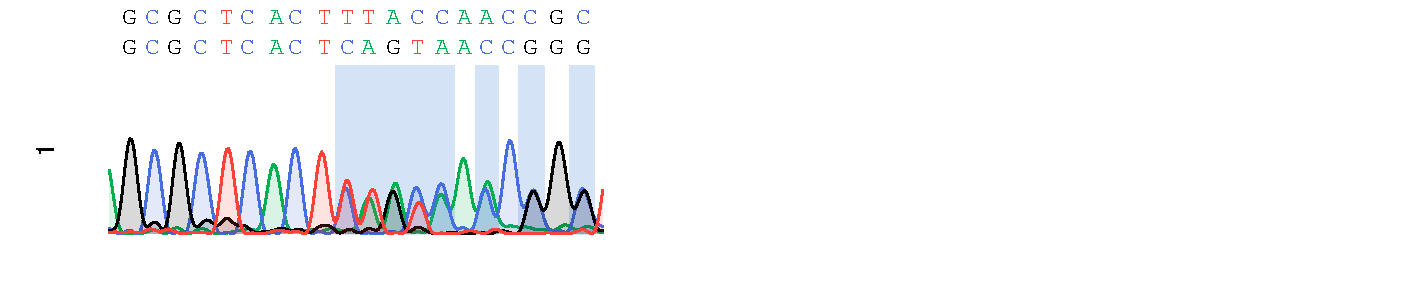
\includegraphics[width=\maxwidth]{figure/chromatogram4-1} 

\end{knitrout}

@

\subsection*{Chromatogram5(height=1.6,width=60)}
\begin{knitrout}
\definecolor{shadecolor}{rgb}{0.969, 0.969, 0.969}\color{fgcolor}\begin{kframe}


{\ttfamily\noindent\bfseries\color{errorcolor}{\#\# Error in par(originalpar): 图形参数"{}pin"{}的值设得不对}}\end{kframe}
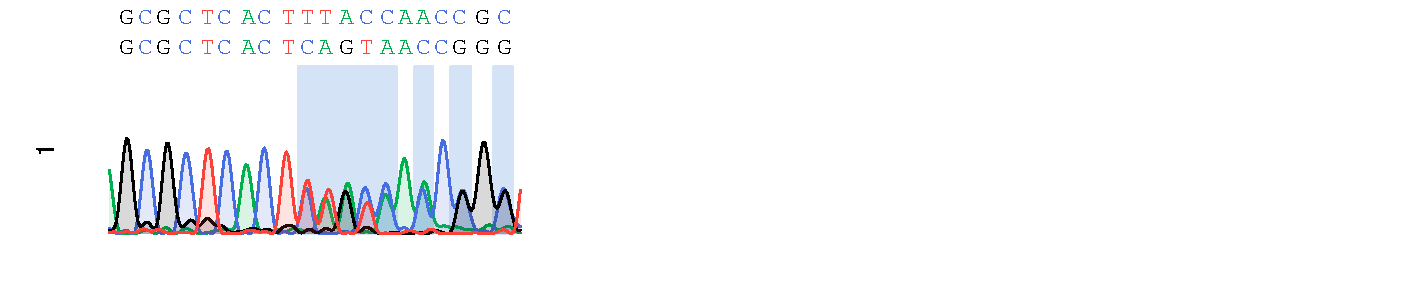
\includegraphics[width=\maxwidth]{figure/chromatogram5-1} 

\end{knitrout}

\newpage
\subsection*{序列比对结果}
\begin{texshade}{./aln.fasta}
\seqtype{N}
\shadingmode[structure]{functional}
\threshold{50}
\showconsensus[ColdHot]{bottom}
\shadingcolors{blues}
\hidelogoscale
\shownames{left}
\nameseq{alle1}{alle1}
\nameseq{alle2}{alle2}
\nameseq{ref}{reference}
\shownumbering{bottom}
\showlegend
\end{texshade}
\end{document}
